\subsection{Class Diagram}

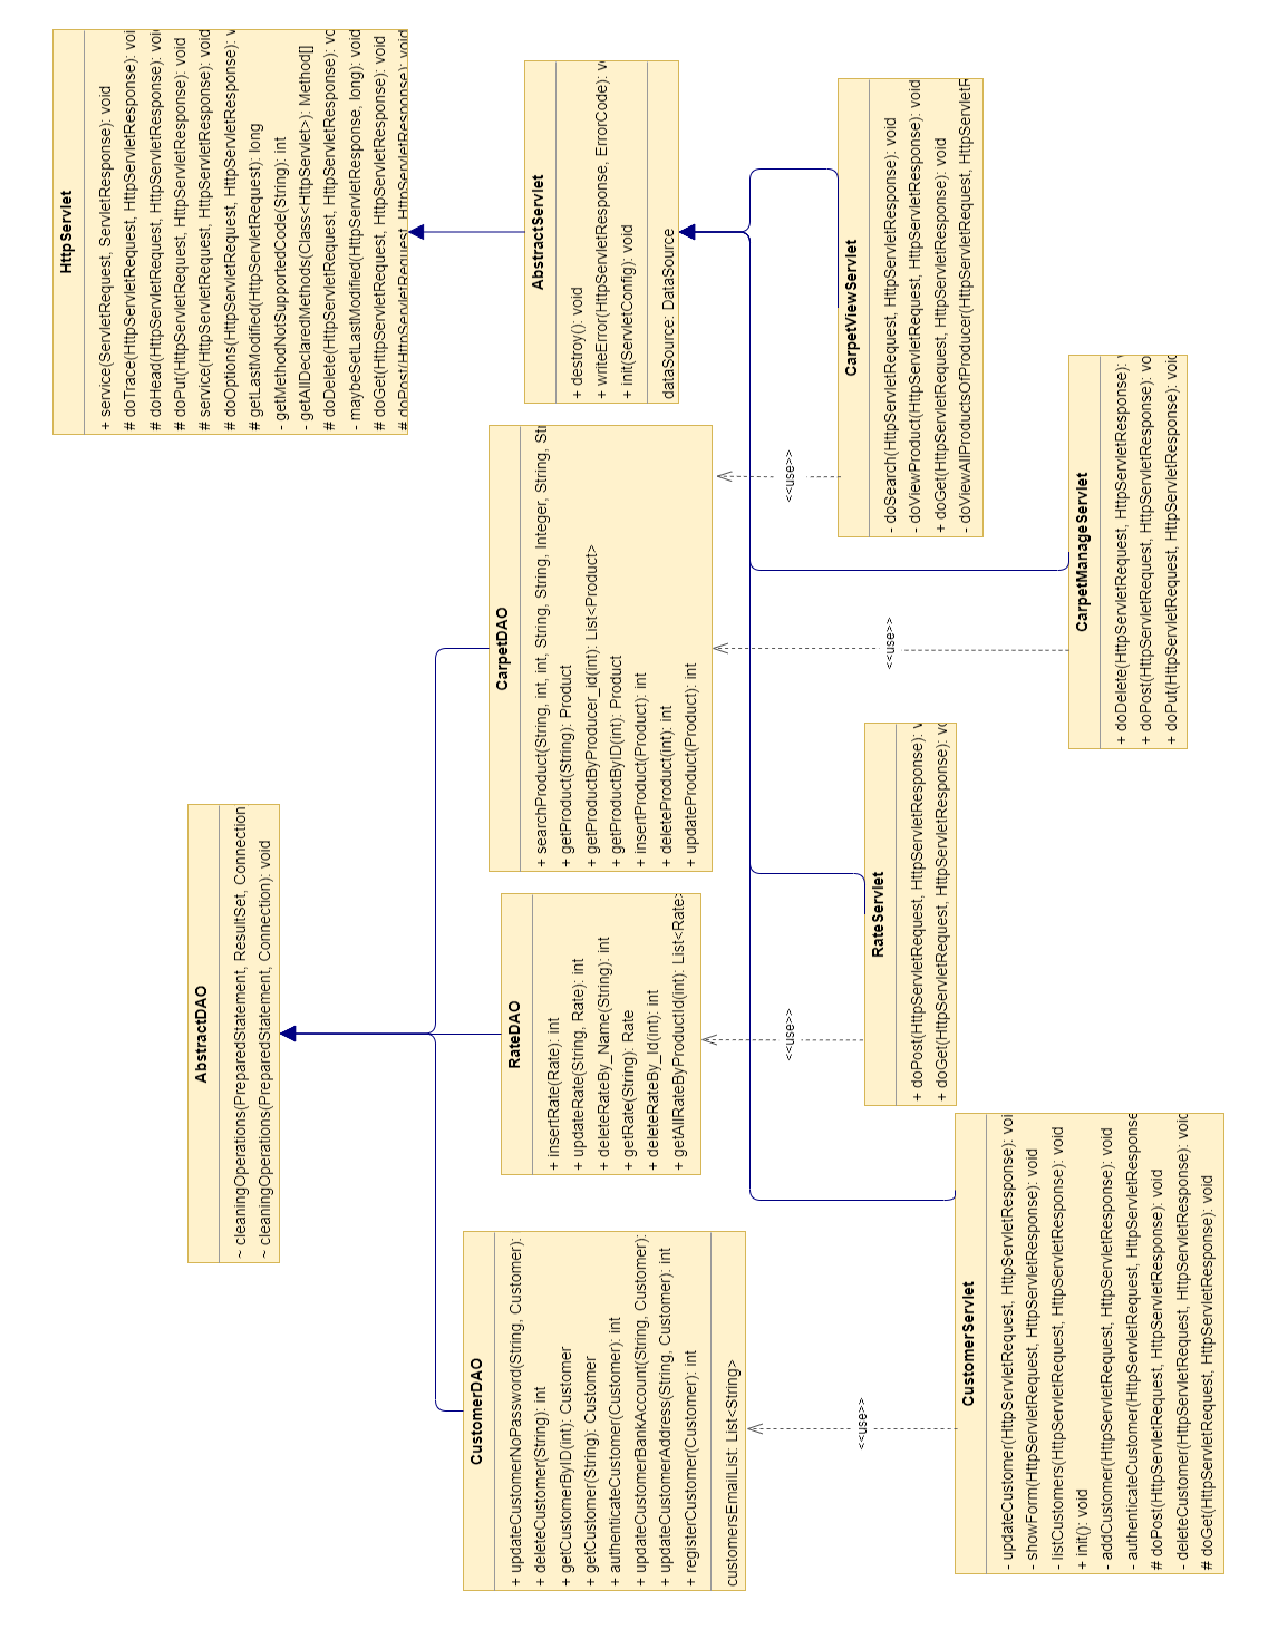
\includegraphics[scale=0.9]{wab-homework1/sections/BLL/classdiagram.pdf}
The class diagram depicts the classes used to manage customers and products (different types of carpets, in our case). Four servlets are described: CustomerServlet, which handles the customer resource, retrieves their information, and allows them to log in and register on the web application; CarpetManageServlet,\\
which handles the products resource and enables producers to create or delete a product, as well as customers to obtain product information; CarpetViewServlet which manages the search and filter process on products; and RateServlet which retrieves the product rating information.\\\\
Each servlet extends the AbstractDatabaseServlet, which is necessary to establish a connection to the database. The customer resource is entirely handled by the CustomerServlet, which implements the doPost and doGet methods. Not all URIs are freely accessible, as only customers or producers\\
can access the URIs to get information about one or more products. Furthermore, some URLs are banned for both users and are only accessible to the site administrator. These authentications are managed in filter files.
Several URIs map to the CarpetViewServlet, so the URIs are parsed to determine the requested method by the customer who uses the CarpetOnlineStore. Two of the operations handled by the CarpetViewServlet are filtering products and retrieving product information.\\\\
The CarpetManageServlet implements the doGet, doPost, and doDelete methods, and is responsible for handling product information retrieval, inserting new products, and deleting old ones. The CarpetDAO class grants access to the current products in the database, \\
creates new ones, or updates existing ones. Additionally, other classes, such as getCarpet(...), are used to retrieve product information given a name.
The RateDAO class allows the insertion of a new product rating into the database and retrieves the product's score, which was voted on by previous customers.
